\section{Evaluace}
V této sekci, s ohledem na doporučený rozsah práce a významnost této kapitoly pro naplnění hlavního cíle práce, \textbf{není naučený model analyticky evaluován}.
V krátkosti jsou diskutovány možnosti pro evaluaci variačního autoenkodéru jakožto generativního modelu.
Samotná kvalita rekonstrukce číslic MNIST je pak ponechána k subjektivnímu srovnání.

Evaluace generativních modelů obecně je komplexní oblastí.
Generativní modely mohou mít spoustu využití a proto je nutné evaluační metriku volit s ohledem na konkrétní sledované využití vzniklého modelu.
Speciálně u modelů variačního autoenkodéru existuje další komplikace při volbě evaluační metriky. Není předem známo rozdělení pravděpodobnosti generující vstupní data (\emph{intractable likelihood}), což komplikuje využití standardního přístupu evaluace vůči testovací sadě dat \cite{Goodfellow2016}.

Pro vzájemné srovnání jednotlivých modelů variačního autoenkodéru lze využít porovnání korespondujících hodnot ELBO (viz \autoref{eq:vae_elbo}).
Pro srovnání modelu variačního autoenkodéru s modelem který nevyužívá enkodér, dekodér modulů – např. síť GAN \cite{Goodfellow2014} – lze využít:

\begin{itemize}
    \item \emph{Importance sampling} dle \textcite{Bartler2019}.
    \item \emph{Fréchet inception distance} dle \textcite{Asperti2020}.
\end{itemize}

\autoref{fig:vae_evaluation} ukazuje schopnost modelu variačního autoenkodéru \textbf{generovat rekonstrukce} které splňují charakteristiky vstupu, ale \textbf{nebyly součástí trénovací množiny}.

\begin{figure}[H]
    \centering
    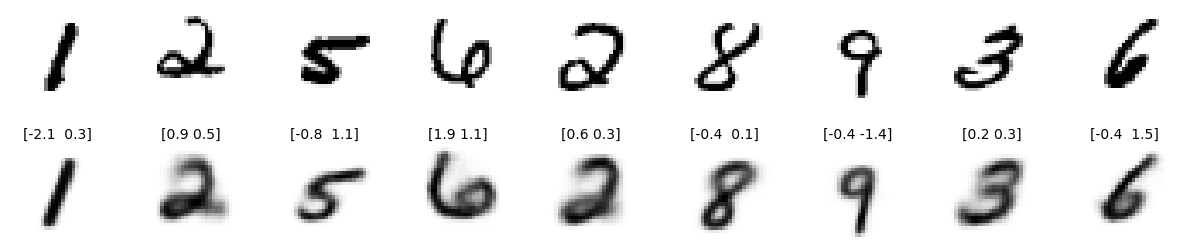
\includegraphics[width=\textwidth]{figures/vae_model_reconstructions.png}
    \caption{Náhodné vzorky z testovací množiny MNIST datasetu $\times$ jejich rekonstrukce vygenerované variačním autoenkodérem. Hodnoty nad rekonstruovanou číslicí udávají souřadnice v latentním prostoru modelu, ze kterých byla tato rekonstrukce dekódována.}
    \label{fig:vae_evaluation}
\end{figure}

Lze pozorovat, že vygenerované rekonstrukce \textbf{odpovídají číslici, která byla poskytnuta jako vstup} a vykazují stejné charakteristiky.
Rekonstrukce jsou rovněž rozostřené. To je důsledek omezení variačního autoenkodéru, které diskutovala \autoref{sec:vae_bluriness}. 

